\documentclass{article}

\usepackage{fancyhdr}
\usepackage{extramarks}
\renewcommand{\thispagestyle}[1]{} % damit Titelseite Kopfzeile bekommt
\usepackage{amsmath}
\usepackage{amsthm}
\usepackage{amsfonts}
\usepackage{tikz}
\usepackage[plain]{algorithm}
\usepackage{algpseudocode}
\usepackage{listings}
\lstset{language=C++, numbers=left, frame=single,}
\usepackage[utf8]{inputenc}
\usepackage{paralist}
\usepackage{multicol}
\usepackage{amssymb}
\usepackage{mathtools}
\usepackage{a4wide}
\usepackage{color}
\usetikzlibrary{arrows}
\usepackage{stmaryrd}
\usepackage{relsize}
\usepackage{qtree}


\usetikzlibrary{automata,positioning}

%
% Basic Document Settings
%

\topmargin=-0.45in
\evensidemargin=0in
\oddsidemargin=0in
\textwidth=6.5in
\textheight=9.0in
\headsep=0.25in

\linespread{1.1}

\pagestyle{fancy}
\lhead{\hmwkGroup\\\hmwkTitle}
\rhead{\hmwkAuthorName}
\lfoot{\lastxmark}
\cfoot{\thepage}

\renewcommand\headrulewidth{0.4pt}
\renewcommand\footrulewidth{0.4pt}

\setlength\parindent{0pt}

%
% Create Problem Sections
%

\newcommand{\enterProblemHeader}[1]{
    \nobreak\extramarks{}{Aufgabe \arabic{#1} wird auf nächster Seite fortgesetzt\ldots}\nobreak{}
    \nobreak\extramarks{Aufgabe \arabic{#1} (fortgesetzt)}{Aufgabe \arabic{#1} wird auf nächster Seite fortgesetzt\ldots}\nobreak{}
}

\newcommand{\exitProblemHeader}[1]{
    \nobreak\extramarks{Aufgabe \arabic{#1} (fortgesetzt)}{Aufgabe \arabic{#1} wird auf nächster Seite fortgesetzt\ldots}\nobreak{}
    \stepcounter{#1}
    \nobreak\extramarks{Aufgabe \arabic{#1}}{}\nobreak{}
}

\setcounter{secnumdepth}{0}
\newcounter{partCounter}
\newcounter{homeworkProblemCounter}
\setcounter{homeworkProblemCounter}{1}
\nobreak\extramarks{Aufgabe \arabic{homeworkProblemCounter}}{}\nobreak{}

%
% Homework Problem Environment
%
% This environment takes an optional argument. When given, it will adjust the
% problem counter. This is useful for when the problems given for your
% assignment aren't sequential. See the last 3 problems of this template for an
% example.
%

\newenvironment{homeworkProblem}[1][-1]{
    \ifnum#1>0
        \setcounter{homeworkProblemCounter}{#1}
    \fi
    \section{Aufgabe \arabic{homeworkProblemCounter}}
    \setcounter{partCounter}{1}
    \enterProblemHeader{homeworkProblemCounter}
}{
    \exitProblemHeader{homeworkProblemCounter}
}

%
% Homework Details
%   - Title
%   - Due date
%   - Class
%   - Section/Time
%   - Instructor
%   - Author
%

\date{29.06.2018}
\newcommand{\hmwkTitle}{Übungsblatt\ \#10}
\newcommand{\hmwkGroup}{Übungsgruppe 16}
\newcommand{\hmwkDueDate}{5. Juli 2018}
\newcommand{\hmwkClass}{Datenstrukturen und Algorithmen}
\newcommand{\hmwkAuthorName}{\textbf{Niklas Hempel (349492), Jan Knichel (377779), Paul Orschau (381085)}}

%
% Title Page
%

\title{
    \vspace{2in}
    \textmd{\textbf{\hmwkClass:\ \hmwkTitle}}\\
    \normalsize\vspace{0.1in}\small{Abgabe\ am\ \hmwkDueDate\ }\\
    \vspace{3in}
}

\author{\hmwkAuthorName}

\renewcommand{\part}[1]{\textbf{\large Part \Alph{partCounter}}\stepcounter{partCounter}\\}

%
% Various Helper Commands
%

% Useful for algorithms
\newcommand{\alg}[1]{\textsc{\bfseries \footnotesize #1}}

% For derivatives
\newcommand{\deriv}[1]{\frac{\mathrm{d}}{\mathrm{d}x} (#1)}

% For partial derivatives
\newcommand{\pderiv}[2]{\frac{\partial}{\partial #1} (#2)}

% Integral dx
\newcommand{\dx}{\mathrm{d}x}

% Alias for the Solution section header
\newcommand{\loesung}{\textbf{\large Lösung}}

% Parts
\newcommand{\teil}[1]{\vspace{15pt}\textbf{Teil #1}}


%
% Start of Document
%

\begin{document}

  \maketitle

  \pagebreak
  
  \begin{homeworkProblem}
    \teil{a)}
    \\Der Algorithmus berechnet einen minimalen zusammenh\"angenden Graphen. Die gr\"o{\ss}ten Kanten, die nicht wichtig sind, um einen zusammenh\"angenden Graphen zu erhalten, werden gel\"oscht.
    \\Dies geht daraus hervor, dass in jeder Schleifeniteration die Kante mit dem gr\"o{\ss}ten Gewicht gel\"oscht wird, falls der Graph danach noch zusammenh\"angend ist.
    $$ $$
    \teil{b)}
    $$ $$
    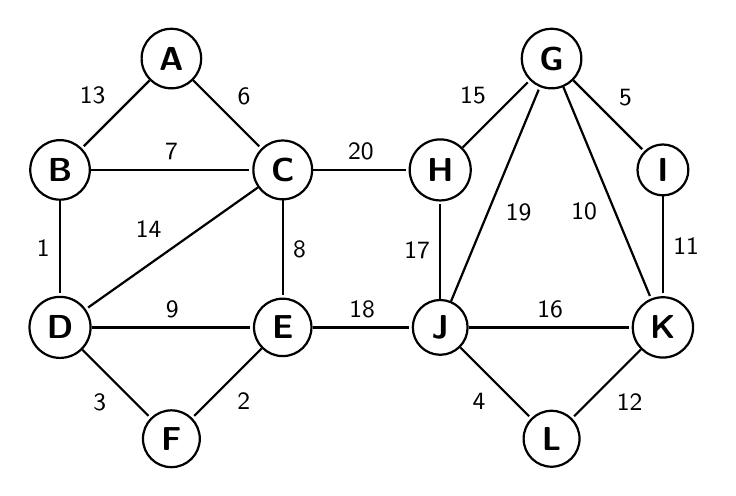
\begin{tikzpicture}[,>=stealth',shorten >=1pt,auto,node distance=2cm,
                        thick,main node/.style={circle,draw,font=\sffamily\large\bfseries}]

      \node[main node] (1) {A};
      \node[main node] (2) [below left of=1] {B};
      \node[main node] (3) [below right of=1] {C};
      \node[main node] (4) [below of=2] {D};
      \node[main node] (5) [below of=3] {E};
      \node[main node] (6) [below left of=5] {F};
      \node[main node] (7) [right of=5] {J};
      \node[main node] (8) [right of=3] {H};
      \node[main node] (9) [above right of=8] {G};
      \node[main node] (10) [below right of=9] {I};
      \node[main node] (11) [below of=10] {K};
      \node[main node] (12) [below right of=7] {L};
      \path[every node/.style={font=\sffamily\small}]
        (1) edge node[above left] {13} (2)
        (1)	edge node {6} (3)
        (2) edge node {7} (3)
        (2) edge node[left] {1} (4)
        (3) edge node {20} (8)
        (3) edge node {8} (5)
        (3) edge node[above left] {14} (4)
        (4) edge node[below left] {3} (6)
        (4) edge node {9} (5)
        (5) edge node {2} (6)
        (5) edge node {18} (7)
        (7) edge node[below left] {4} (12)
        (7) edge node {16} (11)
        (7) edge node {17} (8)
        (7) edge node[below right] {19} (9)
        (8) edge node {15} (9)
        (9) edge node {5} (10)
        (9) edge node[below left] {10} (11)
        (10) edge node {11} (11)
        (11) edge node {12} (12);
    \end{tikzpicture}
    $$ $$
    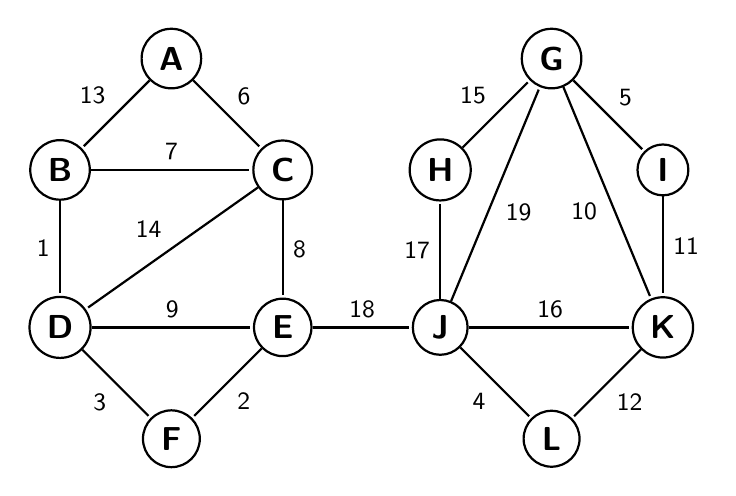
\begin{tikzpicture}[,>=stealth',shorten >=1pt,auto,node distance=2cm,
                        thick,main node/.style={circle,draw,font=\sffamily\large\bfseries}]

      \node[main node] (1) {A};
      \node[main node] (2) [below left of=1] {B};
      \node[main node] (3) [below right of=1] {C};
      \node[main node] (4) [below of=2] {D};
      \node[main node] (5) [below of=3] {E};
      \node[main node] (6) [below left of=5] {F};
      \node[main node] (7) [right of=5] {J};
      \node[main node] (8) [right of=3] {H};
      \node[main node] (9) [above right of=8] {G};
      \node[main node] (10) [below right of=9] {I};
      \node[main node] (11) [below of=10] {K};
      \node[main node] (12) [below right of=7] {L};
      \path[every node/.style={font=\sffamily\small}]
        (1) edge node[above left] {13} (2)
        (1)	edge node {6} (3)
        (2) edge node {7} (3)
        (2) edge node[left] {1} (4)
        (3) edge node {8} (5)
        (3) edge node[above left] {14} (4)
        (4) edge node[below left] {3} (6)
        (4) edge node {9} (5)
        (5) edge node {2} (6)
        (5) edge node {18} (7)
        (7) edge node[below left] {4} (12)
        (7) edge node {16} (11)
        (7) edge node {17} (8)
        (7) edge node[below right] {19} (9)
        (8) edge node {15} (9)
        (9) edge node {5} (10)
        (9) edge node[below left] {10} (11)
        (10) edge node {11} (11)
        (11) edge node {12} (12);
    \end{tikzpicture}
    $$ $$
    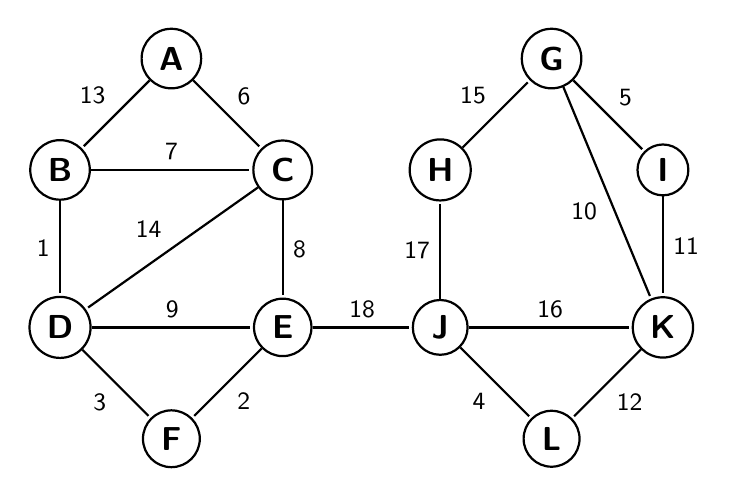
\begin{tikzpicture}[,>=stealth',shorten >=1pt,auto,node distance=2cm,
                        thick,main node/.style={circle,draw,font=\sffamily\large\bfseries}]

      \node[main node] (1) {A};
      \node[main node] (2) [below left of=1] {B};
      \node[main node] (3) [below right of=1] {C};
      \node[main node] (4) [below of=2] {D};
      \node[main node] (5) [below of=3] {E};
      \node[main node] (6) [below left of=5] {F};
      \node[main node] (7) [right of=5] {J};
      \node[main node] (8) [right of=3] {H};
      \node[main node] (9) [above right of=8] {G};
      \node[main node] (10) [below right of=9] {I};
      \node[main node] (11) [below of=10] {K};
      \node[main node] (12) [below right of=7] {L};
      \path[every node/.style={font=\sffamily\small}]
        (1) edge node[above left] {13} (2)
        (1)	edge node {6} (3)
        (2) edge node {7} (3)
        (2) edge node[left] {1} (4)
        (3) edge node {8} (5)
        (3) edge node[above left] {14} (4)
        (4) edge node[below left] {3} (6)
        (4) edge node {9} (5)
        (5) edge node {2} (6)
        (5) edge node {18} (7)
        (7) edge node[below left] {4} (12)
        (7) edge node {16} (11)
        (7) edge node {17} (8)
        (8) edge node {15} (9)
        (9) edge node {5} (10)
        (9) edge node[below left] {10} (11)
        (10) edge node {11} (11)
        (11) edge node {12} (12);
    \end{tikzpicture}
    $$ $$
    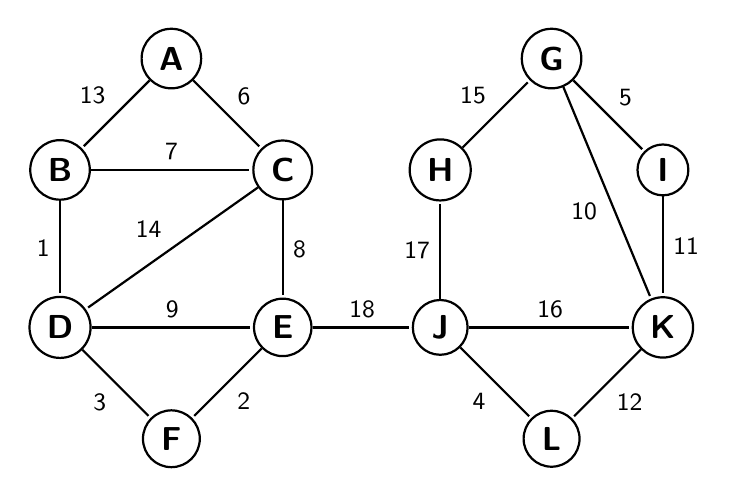
\begin{tikzpicture}[,>=stealth',shorten >=1pt,auto,node distance=2cm,
                        thick,main node/.style={circle,draw,font=\sffamily\large\bfseries}]

      \node[main node] (1) {A};
      \node[main node] (2) [below left of=1] {B};
      \node[main node] (3) [below right of=1] {C};
      \node[main node] (4) [below of=2] {D};
      \node[main node] (5) [below of=3] {E};
      \node[main node] (6) [below left of=5] {F};
      \node[main node] (7) [right of=5] {J};
      \node[main node] (8) [right of=3] {H};
      \node[main node] (9) [above right of=8] {G};
      \node[main node] (10) [below right of=9] {I};
      \node[main node] (11) [below of=10] {K};
      \node[main node] (12) [below right of=7] {L};
      \path[every node/.style={font=\sffamily\small}]
        (1) edge node[above left] {13} (2)
        (1)	edge node {6} (3)
        (2) edge node {7} (3)
        (2) edge node[left] {1} (4)
        (3) edge node {8} (5)
        (3) edge node[above left] {14} (4)
        (4) edge node[below left] {3} (6)
        (4) edge node {9} (5)
        (5) edge node {2} (6)
        (5) edge node {18} (7)
        (7) edge node[below left] {4} (12)
        (7) edge node {16} (11)
        (7) edge node {17} (8)
        (8) edge node {15} (9)
        (9) edge node {5} (10)
        (9) edge node[below left] {10} (11)
        (10) edge node {11} (11)
        (11) edge node {12} (12);
    \end{tikzpicture}
    $$ $$
    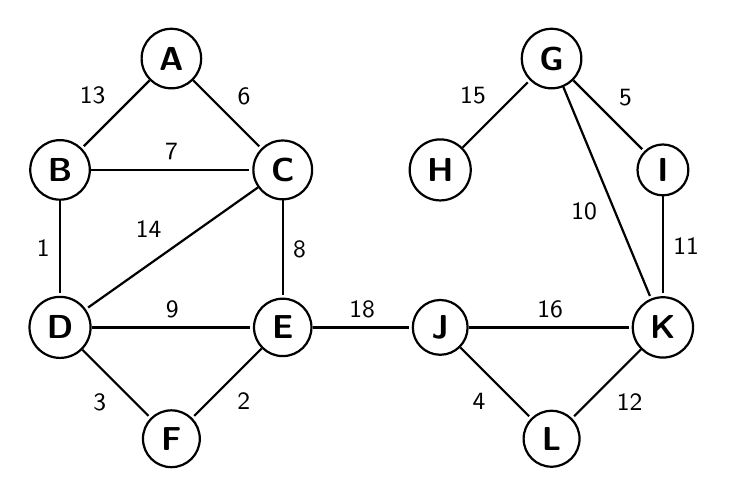
\begin{tikzpicture}[,>=stealth',shorten >=1pt,auto,node distance=2cm,
                        thick,main node/.style={circle,draw,font=\sffamily\large\bfseries}]

      \node[main node] (1) {A};
      \node[main node] (2) [below left of=1] {B};
      \node[main node] (3) [below right of=1] {C};
      \node[main node] (4) [below of=2] {D};
      \node[main node] (5) [below of=3] {E};
      \node[main node] (6) [below left of=5] {F};
      \node[main node] (7) [right of=5] {J};
      \node[main node] (8) [right of=3] {H};
      \node[main node] (9) [above right of=8] {G};
      \node[main node] (10) [below right of=9] {I};
      \node[main node] (11) [below of=10] {K};
      \node[main node] (12) [below right of=7] {L};
      \path[every node/.style={font=\sffamily\small}]
        (1) edge node[above left] {13} (2)
        (1)	edge node {6} (3)
        (2) edge node {7} (3)
        (2) edge node[left] {1} (4)
        (3) edge node {8} (5)
        (3) edge node[above left] {14} (4)
        (4) edge node[below left] {3} (6)
        (4) edge node {9} (5)
        (5) edge node {2} (6)
        (5) edge node {18} (7)
        (7) edge node[below left] {4} (12)
        (7) edge node {16} (11)
        (8) edge node {15} (9)
        (9) edge node {5} (10)
        (9) edge node[below left] {10} (11)
        (10) edge node {11} (11)
        (11) edge node {12} (12);
    \end{tikzpicture}
    $$ $$
    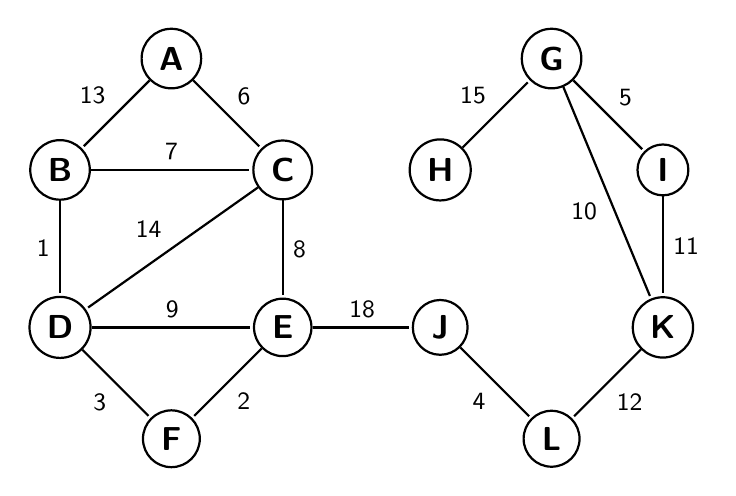
\begin{tikzpicture}[,>=stealth',shorten >=1pt,auto,node distance=2cm,
                        thick,main node/.style={circle,draw,font=\sffamily\large\bfseries}]

      \node[main node] (1) {A};
      \node[main node] (2) [below left of=1] {B};
      \node[main node] (3) [below right of=1] {C};
      \node[main node] (4) [below of=2] {D};
      \node[main node] (5) [below of=3] {E};
      \node[main node] (6) [below left of=5] {F};
      \node[main node] (7) [right of=5] {J};
      \node[main node] (8) [right of=3] {H};
      \node[main node] (9) [above right of=8] {G};
      \node[main node] (10) [below right of=9] {I};
      \node[main node] (11) [below of=10] {K};
      \node[main node] (12) [below right of=7] {L};
      \path[every node/.style={font=\sffamily\small}]
        (1) edge node[above left] {13} (2)
        (1)	edge node {6} (3)
        (2) edge node {7} (3)
        (2) edge node[left] {1} (4)
        (3) edge node {8} (5)
        (3) edge node[above left] {14} (4)
        (4) edge node[below left] {3} (6)
        (4) edge node {9} (5)
        (5) edge node {2} (6)
        (5) edge node {18} (7)
        (7) edge node[below left] {4} (12)
        (8) edge node {15} (9)
        (9) edge node {5} (10)
        (9) edge node[below left] {10} (11)
        (10) edge node {11} (11)
        (11) edge node {12} (12);
    \end{tikzpicture}
    $$ $$
    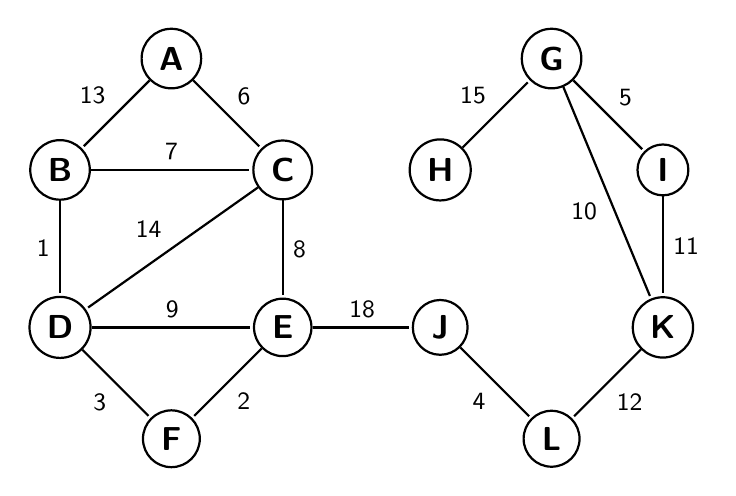
\begin{tikzpicture}[,>=stealth',shorten >=1pt,auto,node distance=2cm,
                        thick,main node/.style={circle,draw,font=\sffamily\large\bfseries}]

      \node[main node] (1) {A};
      \node[main node] (2) [below left of=1] {B};
      \node[main node] (3) [below right of=1] {C};
      \node[main node] (4) [below of=2] {D};
      \node[main node] (5) [below of=3] {E};
      \node[main node] (6) [below left of=5] {F};
      \node[main node] (7) [right of=5] {J};
      \node[main node] (8) [right of=3] {H};
      \node[main node] (9) [above right of=8] {G};
      \node[main node] (10) [below right of=9] {I};
      \node[main node] (11) [below of=10] {K};
      \node[main node] (12) [below right of=7] {L};
      \path[every node/.style={font=\sffamily\small}]
        (1) edge node[above left] {13} (2)
        (1)	edge node {6} (3)
        (2) edge node {7} (3)
        (2) edge node[left] {1} (4)
        (3) edge node {8} (5)
        (3) edge node[above left] {14} (4)
        (4) edge node[below left] {3} (6)
        (4) edge node {9} (5)
        (5) edge node {2} (6)
        (5) edge node {18} (7)
        (7) edge node[below left] {4} (12)
        (8) edge node {15} (9)
        (9) edge node {5} (10)
        (9) edge node[below left] {10} (11)
        (10) edge node {11} (11)
        (11) edge node {12} (12);
    \end{tikzpicture}
    $$ $$
    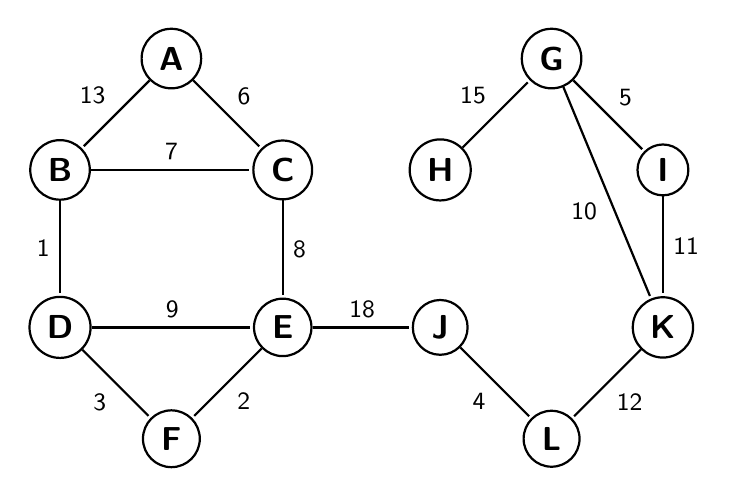
\begin{tikzpicture}[,>=stealth',shorten >=1pt,auto,node distance=2cm,
                        thick,main node/.style={circle,draw,font=\sffamily\large\bfseries}]

      \node[main node] (1) {A};
      \node[main node] (2) [below left of=1] {B};
      \node[main node] (3) [below right of=1] {C};
      \node[main node] (4) [below of=2] {D};
      \node[main node] (5) [below of=3] {E};
      \node[main node] (6) [below left of=5] {F};
      \node[main node] (7) [right of=5] {J};
      \node[main node] (8) [right of=3] {H};
      \node[main node] (9) [above right of=8] {G};
      \node[main node] (10) [below right of=9] {I};
      \node[main node] (11) [below of=10] {K};
      \node[main node] (12) [below right of=7] {L};
      \path[every node/.style={font=\sffamily\small}]
        (1) edge node[above left] {13} (2)
        (1)	edge node {6} (3)
        (2) edge node {7} (3)
        (2) edge node[left] {1} (4)
        (3) edge node {8} (5)
        (4) edge node[below left] {3} (6)
        (4) edge node {9} (5)
        (5) edge node {2} (6)
        (5) edge node {18} (7)
        (7) edge node[below left] {4} (12)
        (8) edge node {15} (9)
        (9) edge node {5} (10)
        (9) edge node[below left] {10} (11)
        (10) edge node {11} (11)
        (11) edge node {12} (12);
    \end{tikzpicture}
    $$ $$
    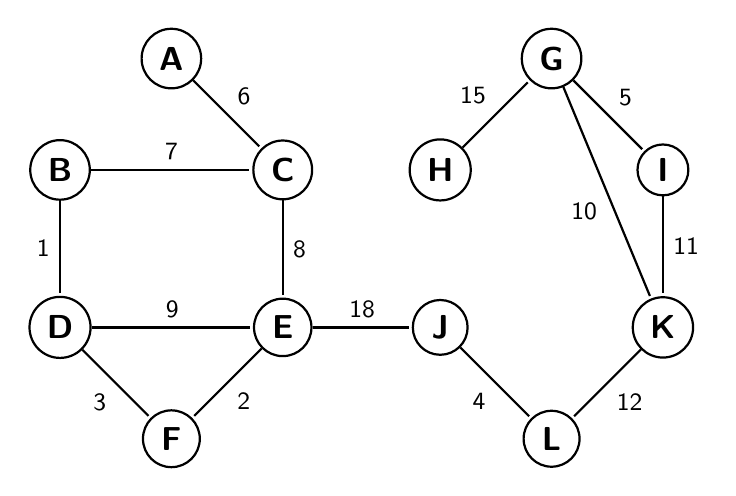
\begin{tikzpicture}[,>=stealth',shorten >=1pt,auto,node distance=2cm,
                        thick,main node/.style={circle,draw,font=\sffamily\large\bfseries}]

      \node[main node] (1) {A};
      \node[main node] (2) [below left of=1] {B};
      \node[main node] (3) [below right of=1] {C};
      \node[main node] (4) [below of=2] {D};
      \node[main node] (5) [below of=3] {E};
      \node[main node] (6) [below left of=5] {F};
      \node[main node] (7) [right of=5] {J};
      \node[main node] (8) [right of=3] {H};
      \node[main node] (9) [above right of=8] {G};
      \node[main node] (10) [below right of=9] {I};
      \node[main node] (11) [below of=10] {K};
      \node[main node] (12) [below right of=7] {L};
      \path[every node/.style={font=\sffamily\small}]
        (1)	edge node {6} (3)
        (2) edge node {7} (3)
        (2) edge node[left] {1} (4)
        (3) edge node {8} (5)
        (4) edge node[below left] {3} (6)
        (4) edge node {9} (5)
        (5) edge node {2} (6)
        (5) edge node {18} (7)
        (7) edge node[below left] {4} (12)
        (8) edge node {15} (9)
        (9) edge node {5} (10)
        (9) edge node[below left] {10} (11)
        (10) edge node {11} (11)
        (11) edge node {12} (12);
    \end{tikzpicture}
    $$ $$
    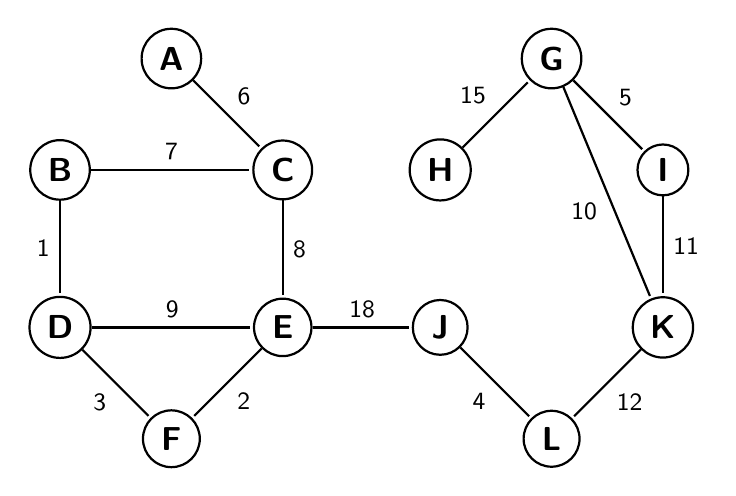
\begin{tikzpicture}[,>=stealth',shorten >=1pt,auto,node distance=2cm,
                        thick,main node/.style={circle,draw,font=\sffamily\large\bfseries}]

      \node[main node] (1) {A};
      \node[main node] (2) [below left of=1] {B};
      \node[main node] (3) [below right of=1] {C};
      \node[main node] (4) [below of=2] {D};
      \node[main node] (5) [below of=3] {E};
      \node[main node] (6) [below left of=5] {F};
      \node[main node] (7) [right of=5] {J};
      \node[main node] (8) [right of=3] {H};
      \node[main node] (9) [above right of=8] {G};
      \node[main node] (10) [below right of=9] {I};
      \node[main node] (11) [below of=10] {K};
      \node[main node] (12) [below right of=7] {L};
      \path[every node/.style={font=\sffamily\small}]
        (1)	edge node {6} (3)
        (2) edge node {7} (3)
        (2) edge node[left] {1} (4)
        (3) edge node {8} (5)
        (4) edge node[below left] {3} (6)
        (4) edge node {9} (5)
        (5) edge node {2} (6)
        (5) edge node {18} (7)
        (7) edge node[below left] {4} (12)
        (8) edge node {15} (9)
        (9) edge node {5} (10)
        (9) edge node[below left] {10} (11)
        (10) edge node {11} (11)
        (11) edge node {12} (12);
    \end{tikzpicture}\\
    $$ $$
    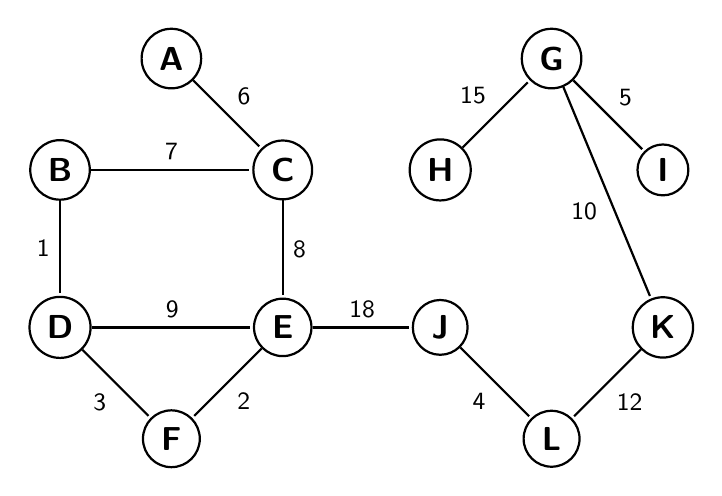
\begin{tikzpicture}[,>=stealth',shorten >=1pt,auto,node distance=2cm,
                        thick,main node/.style={circle,draw,font=\sffamily\large\bfseries}]

      \node[main node] (1) {A};
      \node[main node] (2) [below left of=1] {B};
      \node[main node] (3) [below right of=1] {C};
      \node[main node] (4) [below of=2] {D};
      \node[main node] (5) [below of=3] {E};
      \node[main node] (6) [below left of=5] {F};
      \node[main node] (7) [right of=5] {J};
      \node[main node] (8) [right of=3] {H};
      \node[main node] (9) [above right of=8] {G};
      \node[main node] (10) [below right of=9] {I};
      \node[main node] (11) [below of=10] {K};
      \node[main node] (12) [below right of=7] {L};
      \path[every node/.style={font=\sffamily\small}]
        (1)	edge node {6} (3)
        (2) edge node {7} (3)
        (2) edge node[left] {1} (4)
        (3) edge node {8} (5)
        (4) edge node[below left] {3} (6)
        (4) edge node {9} (5)
        (5) edge node {2} (6)
        (5) edge node {18} (7)
        (7) edge node[below left] {4} (12)
        (8) edge node {15} (9)
        (9) edge node {5} (10)
        (9) edge node[below left] {10} (11)
        (11) edge node {12} (12);
    \end{tikzpicture}
    $$ $$
    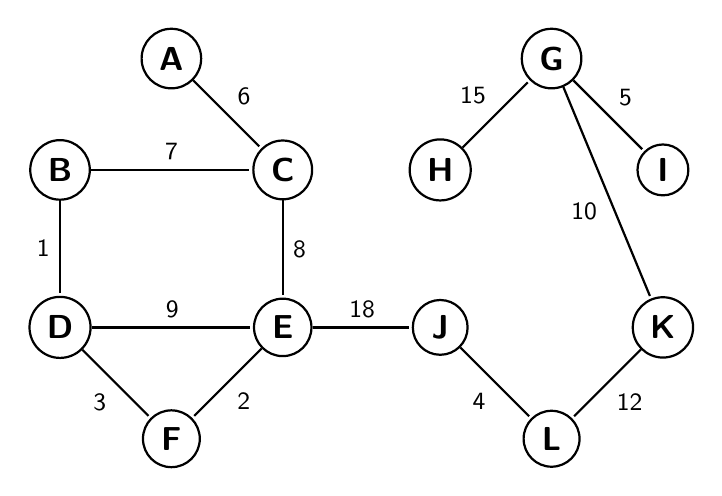
\begin{tikzpicture}[,>=stealth',shorten >=1pt,auto,node distance=2cm,
                        thick,main node/.style={circle,draw,font=\sffamily\large\bfseries}]

      \node[main node] (1) {A};
      \node[main node] (2) [below left of=1] {B};
      \node[main node] (3) [below right of=1] {C};
      \node[main node] (4) [below of=2] {D};
      \node[main node] (5) [below of=3] {E};
      \node[main node] (6) [below left of=5] {F};
      \node[main node] (7) [right of=5] {J};
      \node[main node] (8) [right of=3] {H};
      \node[main node] (9) [above right of=8] {G};
      \node[main node] (10) [below right of=9] {I};
      \node[main node] (11) [below of=10] {K};
      \node[main node] (12) [below right of=7] {L};
      \path[every node/.style={font=\sffamily\small}]
        (1)	edge node {6} (3)
        (2) edge node {7} (3)
        (2) edge node[left] {1} (4)
        (3) edge node {8} (5)
        (4) edge node[below left] {3} (6)
        (4) edge node {9} (5)
        (5) edge node {2} (6)
        (5) edge node {18} (7)
        (7) edge node[below left] {4} (12)
        (8) edge node {15} (9)
        (9) edge node {5} (10)
        (9) edge node[below left] {10} (11)
        (11) edge node {12} (12);
    \end{tikzpicture}
    $$ $$
    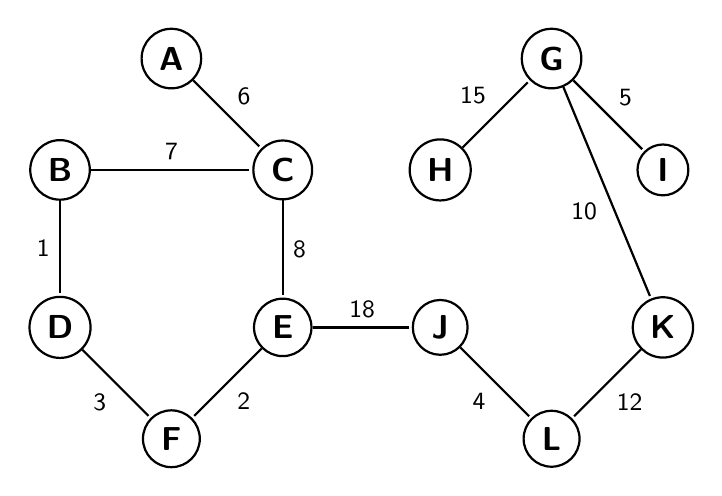
\begin{tikzpicture}[,>=stealth',shorten >=1pt,auto,node distance=2cm,
                        thick,main node/.style={circle,draw,font=\sffamily\large\bfseries}]

      \node[main node] (1) {A};
      \node[main node] (2) [below left of=1] {B};
      \node[main node] (3) [below right of=1] {C};
      \node[main node] (4) [below of=2] {D};
      \node[main node] (5) [below of=3] {E};
      \node[main node] (6) [below left of=5] {F};
      \node[main node] (7) [right of=5] {J};
      \node[main node] (8) [right of=3] {H};
      \node[main node] (9) [above right of=8] {G};
      \node[main node] (10) [below right of=9] {I};
      \node[main node] (11) [below of=10] {K};
      \node[main node] (12) [below right of=7] {L};
      \path[every node/.style={font=\sffamily\small}]
        (1)	edge node {6} (3)
        (2) edge node {7} (3)
        (2) edge node[left] {1} (4)
        (3) edge node {8} (5)
        (4) edge node[below left] {3} (6)
        (5) edge node {2} (6)
        (5) edge node {18} (7)
        (7) edge node[below left] {4} (12)
        (8) edge node {15} (9)
        (9) edge node {5} (10)
        (9) edge node[below left] {10} (11)
        (11) edge node {12} (12);
    \end{tikzpicture}
    $$ $$
    \textbf{8-mal:}
    \\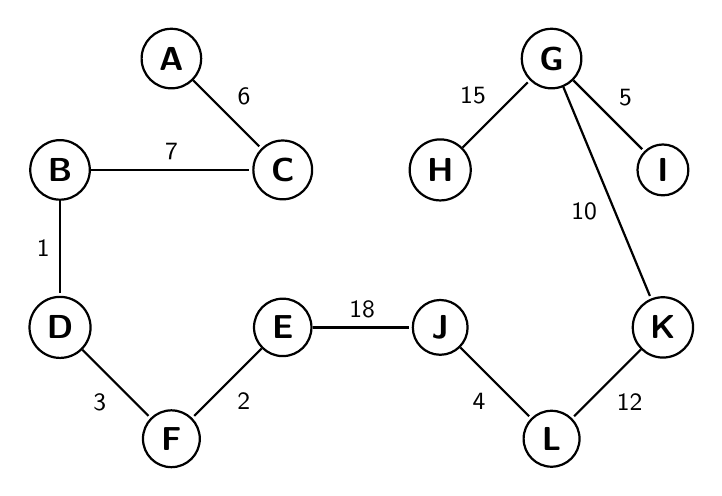
\begin{tikzpicture}[,>=stealth',shorten >=1pt,auto,node distance=2cm,
                        thick,main node/.style={circle,draw,font=\sffamily\large\bfseries}]

      \node[main node] (1) {A};
      \node[main node] (2) [below left of=1] {B};
      \node[main node] (3) [below right of=1] {C};
      \node[main node] (4) [below of=2] {D};
      \node[main node] (5) [below of=3] {E};
      \node[main node] (6) [below left of=5] {F};
      \node[main node] (7) [right of=5] {J};
      \node[main node] (8) [right of=3] {H};
      \node[main node] (9) [above right of=8] {G};
      \node[main node] (10) [below right of=9] {I};
      \node[main node] (11) [below of=10] {K};
      \node[main node] (12) [below right of=7] {L};
      \path[every node/.style={font=\sffamily\small}]
        (1)	edge node {6} (3)
        (2) edge node {7} (3)
        (2) edge node[left] {1} (4)
        (4) edge node[below left] {3} (6)
        (5) edge node {2} (6)
        (5) edge node {18} (7)
        (7) edge node[below left] {4} (12)
        (8) edge node {15} (9)
        (9) edge node {5} (10)
        (9) edge node[below left] {10} (11)
        (11) edge node {12} (12);
    \end{tikzpicture}
  \end{homeworkProblem}
  
  \pagebreak
  
  \begin{homeworkProblem}
    
    "Der minimale Spannbaum eines Graphen, dessen Kantengewichte alle paarweise verschieden sind ist eindeutig."
    $$ $$
    \textbf{Beweis:} Durch Widerspruch
    \\ Angenommen, der minimale Spannbaum eines solchen Graphen wäre nicht eindeutig. Dann gäbe es mindestens zwei minimale Spannbäume, $A$ und $B$. Da $A$ und $B$ unterschiedlich sind, muss es Kanten geben, die in einem der beiden Bäume, aber nicht im anderen enthalten sind. Da alle Kantengewichte paarweise verschieden sind, können wir unter all diesen Kanten diejenige mit dem niedrigsten Kantengewicht eindeutig auswählen und $a$ nennen.
    \\ O.B.d.A. sei $a$ in $A$ und nicht in $B$, ansonsten benenne die Graphen um.
    \\ Da $B$ auch ein Spannbaum ist, muss $B \cup a$ einen Kreis $C$ enthalten. $A$ (als Spannbaum) hat keine Kreise, daher muss $C$ eine Kante $b$ enthalten, die nicht in $A$ enthalten ist. Weil wir festgelegt haben, dass $a$ in $A$ liegt, müssen $b$ und $a$ zwei unterschiedliche Kanten sein. $b$ kann also nur in $B$ liegen.
    \\ Da $a$ die Kante mit dem kleinsten Kantengewicht ist, die nur in einem der beiden Graphen enthalten ist, muss $W(a) < W(c)$ gelten, denn alle Kantengewichte sind paarweise verschieden. Ersetzt man in $B$ die Kante $b$ durch $a$, ist der resultierende Spannbaum $B'$ kleiner als $B$. Dies widerspricht der Annahme, dass $B$ ein minimaler Spannbaum war, und damit ist die ursprüngliche These bewiesen. \qed
    
  \end{homeworkProblem}
  
  \begin{homeworkProblem}
    
    1. $h(v) = \| K(v)-K(t) \|_{1}$
    \\ Gegenbeispiel:
    $$ $$
    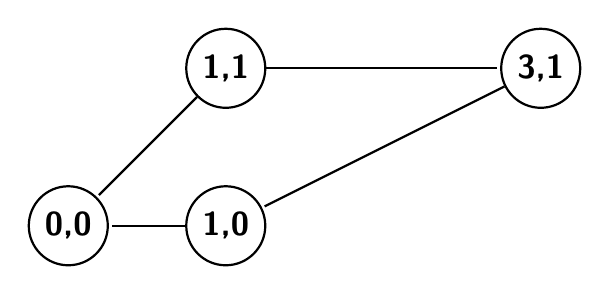
\begin{tikzpicture}[,>=stealth',shorten >=1pt,auto,node distance=2cm,
                        thick,main node/.style={circle,draw,font=\sffamily\large\bfseries}]

      \node[main node] (1) {1,1};
      \node[main node] (2) [below of=1] {1,0};
      \node[main node] (3) [left of=2] {0,0};
      \node[main node] (4) [right of=1, xshift=2cm] {3,1};
      \path[every node/.style={font=\sffamily\small}]
        (1) edge node {} (4)
        	edge node {} (3)
        (2) edge node {} (3)
        (4) edge node {} (2);
    \end{tikzpicture}
    $$ $$
    Es gibt zwei M\"oglichkeiten, von $s(0,0)$ zu $t(3,1)$ zu gelangen. Einmal \"uber $v'(1,1)$ oder \"uber $v''(1,0)$.
    \\1) \"uber $v'$: $\sqrt{1^2+1^2} + 2 = \sqrt{2} + 2 \approx 3,41$
    \\2) \"uber $v''$: $\sqrt{2^2+1^2} + 1 = \sqrt{5} + 1 \approx 3,24$
    \\ \texttt{ExtractMin} w\"alt nun das Minimum der Funktion  $h(v) = \| K(v)-K(t) \|_{1} + dist(v)$ aus.
    \\F\"ur $v'$ ist dies:
    $$ \| K(v') -K(t) \|_{1} + dist(v') = \left\| \left(\begin{array}{c} 1-3 \\ 1-1 \end{array}\right) \right\| _{1} + \sqrt{2} = 2 + 0 + \sqrt{2} = 2 + \sqrt{2}$$
    F\"ur $v''$ ist dies:
    $$ \| K(v'') -K(t) \|_{1} + dist(v'') = \left\| \left(\begin{array}{c} 1-3 \\ 0-1 \end{array}\right) \right\| _{1} + 1 = 2 + 1 + 1 = 4 $$
    Da $4 > 2+ \sqrt{2}$ w\"urde hier der Weg \"uber $v'$ gew\"ahlt werde, der Weg \"uber $v''$ ist aber, wie oben berechnet, k\"urzer.  

    \newpage

    2. $h(v) = \| K(v)-K(t) \|_{\infty}$
    \\Der klassische Dijkstra-Algorithmus berechnet den k\"urzesten Abstand von Knoten $s$ zu anderen beliebigen Knoten.
    \\Hier flie{\ss}t nun statt der min. Distanz $dist(v)$ zum Startknoten $s$ auch der minimale Abstand (als Maximumnorm) zum gesuchten Endknoten ein. Die Maximumnorm gibt den Abstand zwischen $v$ und dem Zielknoten $t$ in vertikaler oder horizontaler Ebene zur\"uck, je nachdem, welcher gr\"o{\ss}er ist. Dies entspricht dem minimalen m\"oglichen Abstand zwischen diesen Knoten ($v$ und $t$ liegen auf einer H\"ohe/Breite), bzw. der gr\"o{\ss}ten Kathete des Dreiecks:

    \begin{tikzpicture} 
      \draw(0,0)node[left]{v}--(2,0)node[right]{}--(2,2)node[above]{t}--cycle; 
      \path (0,0)--node[below]{$v_{1}-t_{1}$}(2,0)--node[right]{$v_{2}-t_{2}$}(2,2); 
    \end{tikzpicture} 
    \\Da nun das Minimum der Funktion $ \| K(v)-K(t) \|_{\infty}+ dist(v)$ gesucht wird, findet man genau den Knoten $v$, f\"ur den die Distanz von $v$ zu $s$ addiert mit dem kleinsten m\"oglichen Luftlinienabstand (= die gr\"o{ss}te Kathetenl\"ange) ($v_{1}-t_{1}$ oder $v_{2}-t_{2}$) minimal wird.
    \\Wird die gr\"o{ss}te Kathetenl\"ange minimiert, wird auch die Hypotenuse minimiert, die der euklidschen Norm, bzw. dem Luftlinienabstand entspricht, der hier als unteres Ma{\ss} f\"ur das Gewicht definiert ist.
    \\Es gilt:
    \begin{equation}
    \begin{split}
    & min_{v \in Q} \;\;\; \| K(v)-K(t) \|_{\infty}+ dist(v) \\
    & =  min_{v \in Q} \;\;\; max((v_{1}-t_{1}),(v_{2}-t_{2})) + dist(v) \\
    & \overset{(*)}{\leq}   min_{v \in Q} \;\;\; \sqrt{(v_{1}-t_{1})^2 + (v_{2}-t_{2})^2} + dist(v) \\
    & =  min_{v \in Q} \;\;\; \| K(v) - K(t) \|_{2} +dist(v) \\
    & \leq  min_{v \in Q} \;\;\; W(v,t) + dist(v) \\
    & = dist(t)
    \end{split}
    \end{equation} 
    Vom Startknoten ausgehend wird also immer der bestm\"ogliche Nachfolger gefunden, bis man den Zielknoten $t$ erreicht, den k\"urzesten Weg gefunden hat und der Algorithmus terminiert.
    $$ $$
    $$ $$
    mit $(*)$:
    $$ \|x\|_{\infty} = \sqrt{( \|x\|_{\infty} )^2 } = \sqrt{|x_{max}|^2} \leq \sqrt{|x_{1}|^2 + ... + |x_{n}|^2} = \|x\|_{2}$$
    
  \end{homeworkProblem}

  \pagebreak

  \begin{homeworkProblem}
    
    Das Problem lässt sich durch einen ungerichteten Graphen darstellen, bei dem jede Kante einer \textbf{Verschiebung} im Puzzle entsprich und jeder Knoten einen \textbf{eindeutigen Zustand des Puzzles} beschreibt. Der abgebildete Zustand eines 3x3 Puzzles wäre ein Knoten in diesem Graph, vom dem genau 3 Kanten ausgehen, jeweils für das Verschieben des Puzzleteils 2, 7 oder 4. Jeder Knoten im Graph kann höchstens 4 adjazente Knoten haben, da zu jedem Zeitpunkt nur höchstens 4 nächste Verschiebungen möglich sind. Der Graph ist ungerichtet, da sich jeder Zug immer rückgängig machen lässt.
    $$ $$
    Um das Problem zu lösen, muss man den aktuellen Zustand des Puzzles als Knoten im zugehörigen Graphen finden (s), und dann den gewünschten Zielzustand bzw. -knoten ausfindig machen (t). Hat man beide Knoten, so lässt sich das Problem mit einem Single-Source Shortest Path Algorithmus wie z.B. Dijktra lösen, die Lösung ist der kürzeste Pfad zwischen den Knoten/Zuständen, denn er verwendet möglichst wenige Züge/Verschiebungen/Kanten.
    $$ $$
    Jedes der $n^2-1$ Puzzleteile sowie die "Lücke" brauchen eine eindeutige Position auf dem Schiebebrett. Jede Anordnung ist erlaubt. Für das erste Teil gibt es $n^2$ mögliche Positionen, für das nächste nur noch $n^2-1$ Positionen, usw. bis irgendwann das letzte Stück nur noch $2$ mögliche Positionen hat, die Lücke ist danach eindeutig festgelegt. Die Anzahl von möglichen Zuständen errechnet sich also durch:
    
    \begin{equation}
      n^2 * (n^2-1) * (n^2-3) * \dots * 2 * 1 = n^2!
    \end{equation}
    
  \end{homeworkProblem}
  
  \begin{homeworkProblem}
    
    $$ $$
    \begin{tabular}{c|c|c|c|c|c|c|c}
    	  & A & D & E & B & F & G & H \\
    	\hline
    	A & 0 & 0 & 0 & 0 & 0 & 0 & 0 \\
    	\hline
    	B & 6 & 6 & 6 & 6 & 6 & 6 & 6 \\
    	\hline
    	C & $\infty$ & $\infty$ & $\infty$ & 17 & 17 & 17 & 17 \\
    	\hline
    	D & 3 & 3 & 3 & 3 & 3 & 3 & 3 \\
    	\hline
    	E & 3 & 3 & 3 & 3 & 3 & 3 & 3 \\
    	\hline
    	F & $\infty$ & 6 & 6 & 6 & 6 & 6 & 6 \\
    	\hline
    	G & $\infty$ & 12 & 7 & 7 & 7 & 7 & 7 \\
    	\hline
    	H & $\infty$ & 11 & 11 & 11 & 11 & 11 & 11 \\
    \end{tabular}

  \end{homeworkProblem}
  
  \pagebreak
  
  \begin{homeworkProblem}
    
    $$ $$
    \begin{tabular}{c|c|c|c|c|c|c|c|c|c|c|c|c|c}
    	  & A & B & C & D & E & F & G & H & I & J & K & L & M \\
    	\hline
    	1 & \underline{0} & $\infty$ & $\infty$ & $\infty$ & $\infty$ & $\infty$ & $\infty$ & $\infty$ & $\infty$ & $\infty$ & $\infty$ & $\infty$ & $\infty$ \\
    	\hline
    	2 & 0 & 4 & 3 & $\infty$ & $\infty$ & 9 & $\infty$ & $\infty$ & $\infty$ & \underline{1} & $\infty$ & $\infty$ & $\infty$ \\
    	\hline
    	3 & 0 & 4 & \underline{3} & $\infty$ & $\infty$ & 9 & $\infty$ & $\infty$ & $\infty$ & 1 & $\infty$ & $\infty$ & $\infty$ \\
    	\hline
    	4 & 0 & 4 & 3 & 4 & \underline{3} & 9 & $\infty$ & $\infty$ & $\infty$ & 1 & $\infty$ & $\infty$ & $\infty$ \\
    	\hline
    	5 & 0 & \underline{4} & 3 & 4 & 3 & 5 & $\infty$ & $\infty$ & $\infty$ & 1 & $\infty$ & $\infty$ & $\infty$ \\  
    	\hline
    	6 & 0 & 4 & 3 & 4 & 3 & 5 & $\infty$ & \underline{3} & 3 & 1 & $\infty$ & $\infty$ & $\infty$ \\
    	\hline
    	7 & 0 & 4 & 3 & 4 & 3 & 5 & $\infty$ & 3 & \underline{3} & 1 & $\infty$ & $\infty$ & $\infty$ \\
    	\hline
    	8 & 0 & 4 & 3 & \underline{4} & 3 & 5 & $\infty$ & 3 & 3 & 1 & $\infty$ & $\infty$ & $\infty$ \\
    	\hline
    	9 & 0 & 4 & 3 & 4 & 3 & 5 & \underline{3} & 3 & 3 & 1 & $\infty$ & $\infty$ & $\infty$ \\
    	\hline
    	10 & 0 & 4 & 3 & 4 & 3 & \underline{5} & 3 & 3 & 3 & 1 & $\infty$ & $\infty$ & $\infty$ \\   
    	\hline
    	11 & 0 & 4 & 3 & 4 & 3 & 5 & 3 & 3 & 3 & 1 & \underline{4} & $\infty$ & 4 \\
    	\hline
    	12 & 0 & 4 & 3 & 4 & 3 & 5 & 3 & 3 & 3 & 1 & 4 & 4 & \underline{3} \\
    	\hline
    	13 & 0 & 4 & 3 & 4 & 3 & 5 & 3 & 3 & 3 & 1 & 4 & \underline{4} & 3 \\
    \end{tabular}
    $$ $$
    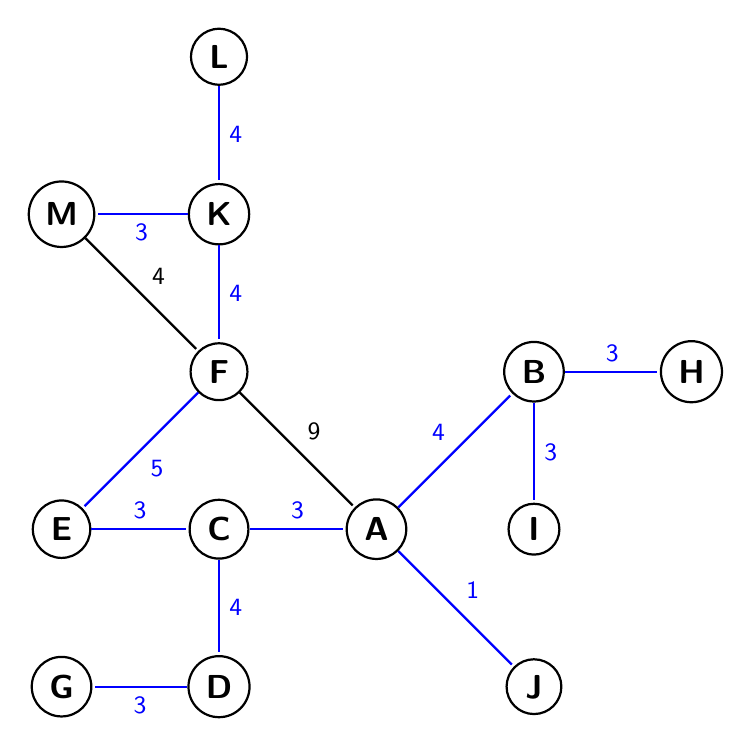
\begin{tikzpicture}[,>=stealth',shorten >=1pt,auto,node distance=2cm,
                        thick,main node/.style={circle,draw,font=\sffamily\large\bfseries}]

      \node[main node] (1) {L};
      \node[main node] (2) [below of=1] {K};
      \node[main node] (3) [left of=2] {M};
      \node[main node] (4) [below of=2] {F};
      \node[main node] (5) [below of=4] {C};
      \node[main node] (6) [left of=5] {E};
      \node[main node] (7) [below of=5] {D};
      \node[main node] (8) [left of=7] {G};
      \node[main node] (9) [right of=5] {A};
      \node[main node] (10) [right of=9] {I};
      \node[main node] (11) [above of=10] {B};
      \node[main node] (12) [right of=11] {H};
      \node[main node] (13) [below of=10] {J};
      \path[every node/.style={font=\sffamily\small}]
        (1) edge[blue] node {4} (2)
        (2)	edge[blue] node {3} (3)
        (2) edge[blue] node {4} (4)
        (3) edge node {4} (4)
        (4) edge[blue] node {5} (6)
        (4) edge node {9} (9)
        (6) edge[blue] node {3} (5)
        (5) edge[blue] node {3} (9)
        (5) edge[blue] node {4} (7)
        (7) edge[blue] node {3} (8)
        (9) edge[blue] node {1} (13)
        (9) edge[blue] node {4} (11)
        (11) edge[blue] node {3} (10)
        (11) edge[blue] node {3} (12);
    \end{tikzpicture}

  \end{homeworkProblem}

\end{document}